% !TeX program = pdflatex
% !TeX encoding = UTF-8
\documentclass[11pt,aspectratio=169,t]{beamer}
% Все презентации курса компилируются только pdflatex.
\usepackage{iftex}
\RequirePDFTeX
\usepackage{cmap}
\usepackage[T2A]{fontenc}
\usepackage[utf8]{inputenc}
\usepackage[english,russian]{babel}
\usepackage{PTSerif}
\usepackage{amsmath,amsfonts,amssymb}
\usepackage{graphicx,microtype,anyfontsize,tikz}
\usepackage{ragged2e}
\usetikzlibrary{arrows.meta,calc}

\usetheme{default}
\usefonttheme{serif}
\DeclareMathOperator{\sen}{sen}
\bibliographystyle{apalike}

% Общие сведения; номер лекции, её название и дата задаются в N.tex.
\newcommand{\coursename}{Введение в маневрирование КА}
\author{Чиняев Владимир Николаевич}
\institute{Московский физико-технический институт}

% Книжное оформление с голубым акцентом.
\definecolor{coursepaper}{HTML}{FBF9F3}
\definecolor{courseink}{HTML}{302B28}
\definecolor{courseaccent}{HTML}{187AA5}
\definecolor{coursemuted}{HTML}{6D6560}
\definecolor{courserule}{HTML}{A9CADA}
\definecolor{coursetint}{HTML}{EDF4F6}
\tikzset{
  course diagram/.style={font=\fontsize{9.5}{11.5}\selectfont,
    line cap=round,line join=round,>=Latex},
  orbit line/.style={draw=courseaccent,line width=1pt},
  aux line/.style={draw=courserule,line width=.5pt},
  vector line/.style={draw=courseink,line width=.65pt,->},
  angle line/.style={draw=courseaccent,line width=.8pt,->},
  orbit point/.style={circle,fill=courseaccent,inner sep=1.7pt}
}
\setbeamercolor{normal text}{fg=courseink,bg=coursepaper}
\setbeamercolor{background canvas}{bg=coursepaper}
\setbeamercolor{structure}{fg=courseaccent}
\setbeamercolor{alerted text}{fg=courseaccent}
\setbeamercolor{frametitle}{fg=courseink,bg=coursepaper}
\setbeamercolor{footline}{fg=coursemuted,bg=coursepaper}
\setbeamercolor{caption name}{fg=courseaccent}

% Основной текст — 11/14 pt; подписи к рисункам — 9.5/11.5 pt.
\let\coursenormalsize\normalsize
\renewcommand{\normalsize}{\coursenormalsize\fontsize{11}{14}\selectfont}
\setbeamerfont{normal text}{size*={11pt}{14pt}}
\setbeamerfont{frametitle}{size*={20pt}{23pt},series=\mdseries}
\setbeamerfont{title}{size*={27pt}{31pt},series=\mdseries}
\setbeamerfont{subtitle}{size*={12.8pt}{15pt},series=\mdseries}
\setbeamerfont{author}{size*={10.8pt}{13pt}}
\setbeamerfont{institute}{size*={9.2pt}{11pt}}
\setbeamerfont{date}{size*={9pt}{11pt}}
\setbeamerfont{footline}{size*={6.8pt}{8pt}}
\setbeamerfont{caption}{size*={9.5pt}{11.5pt}}
\setbeamerfont{itemize/enumerate body}{size*={11pt}{14pt}}
\setbeamerfont{itemize/enumerate subbody}{size*={11pt}{14pt}}
\setbeamerfont{itemize/enumerate subsubbody}{size*={11pt}{14pt}}
\AtBeginDocument{\normalsize}

\setbeamersize{text margin left=6mm,text margin right=6mm}
\setbeamertemplate{navigation symbols}{}
\setbeamertemplate{headline}{}
\setbeamertemplate{caption}[numbered]
\setbeamertemplate{itemize items}[circle]

% Стандартные блоки Beamer позволяют группировать текст и формулы.
\setbeamertemplate{blocks}[default]
\setbeamerfont{block title}{size*={11pt}{14pt},series=\bfseries}
\setbeamerfont{block body}{size*={11pt}{14pt}}
\setbeamercolor{block title}{fg=courseaccent,bg=coursepaper}
\setbeamercolor{block body}{fg=courseink,bg=coursetint}
\setbeamercolor{block title alerted}{parent=block title}
\setbeamercolor{block body alerted}{parent=block body}
\setbeamercolor{block title example}{parent=block title}
\setbeamercolor{block body example}{parent=block body}

% Компактный заголовок; его высота учитывается при размещении содержания.
\setbeamertemplate{frametitle}{%
  \vskip4.5mm%
  \begin{beamercolorbox}[wd=\textwidth,sep=0pt]{frametitle}
    \usebeamerfont{frametitle}\strut\insertframetitle\strut\par
    \vskip2mm%
    {\color{courseaccent}\hrule height .55pt}
  \end{beamercolorbox}%
}

% Нижний колонтитул: курс слева, лекция и номер слайда справа.
\setbeamertemplate{footline}{%
  \begin{beamercolorbox}[wd=\paperwidth,ht=5.5mm,dp=0pt]{footline}
    \begin{tikzpicture}[remember picture,overlay,x=1mm,y=1mm]
      \begin{scope}[shift={(current page.south west)}]
        \draw[courserule,line width=.3pt] (6,5.5)--(154,5.5);
        \node[text=coursemuted,anchor=west,inner sep=0pt,
          font=\usebeamerfont{footline}] at (6,2.8) {\coursename};
        \node[text=coursemuted,anchor=east,inner sep=0pt,
          font=\usebeamerfont{footline}] at (154,2.8)
          {Лекция \arabic{lecture}\quad\textbullet\quad\insertframenumber};
      \end{scope}
    \end{tikzpicture}%
  \end{beamercolorbox}%
}

% Титульник рассчитан на 16:9 (160 × 90 мм), без нижнего колонтитула.
\setbeamertemplate{title page}{%
  \begin{tikzpicture}[remember picture,overlay,x=1mm,y=1mm]
    \begin{scope}[shift={(current page.south west)}]
      \node[text=coursemuted,anchor=north,font=\usebeamerfont{institute}]
        at (80,82) {\insertinstitute};
      \draw[courseaccent,line width=.55pt] (71,71)--(89,71);
      \node[text=courseink,align=center,text width=125mm,
        font=\usebeamerfont{title}] at (80,53)
        {\hyphenpenalty=10000\coursename\par};
      \node[text=courseaccent,align=center,text width=145mm,font=\usebeamerfont{subtitle}]
        at (80,32) {Лекция \arabic{lecture}. \inserttitle};
      \node[text=courseink,font=\usebeamerfont{author}]
        at (80,19) {\insertauthor};
      \node[text=coursemuted,font=\usebeamerfont{date}]
        at (80,9) {\insertdate};
    \end{scope}
  \end{tikzpicture}%
}

\usepackage{booktabs,array}
\setlength{\abovedisplayskip}{5pt}
\setlength{\belowdisplayskip}{5pt}
\setlength{\abovedisplayshortskip}{3pt}
\setlength{\belowdisplayshortskip}{4pt}
\newcommand{\eqcompact}{\fontsize{10}{12}\selectfont}
\newcommand{\figcaption}[1]{{\usebeamerfont{caption}\color{coursemuted}#1\par}}
\newcommand{\derivationmathspacing}{%
  \setlength{\abovedisplayskip}{2pt}%
  \setlength{\belowdisplayskip}{3pt}%
  \setlength{\abovedisplayshortskip}{2pt}%
  \setlength{\belowdisplayshortskip}{2pt}%
  \setlength{\jot}{2pt}}
\newcommand{\vect}[1]{\boldsymbol{#1}}
\setcounter{lecture}{8}
\title{Моделирование последовательности\\протяжённых манёвров с возмущениями}
\date{10 ноября 2026 г.}
% Generated by circular_burn.py. Constant acceleration; no mass or J2.
\newcommand{\CircRadius}{7000}
\newcommand{\CircVelocity}{7{,}546053}
\newcommand{\CircPeriodMinutes}{97{,}142}
\newcommand{\CircDVMps}{1}
\newcommand{\CircLinearDAMeters}{1855{,}27}
\newcommand{\CircLinearEccentricity}{2{,}650392\cdot10^{-4}}
\newcommand{\CircHalfOrbitMinutes}{48{,}571}
\newcommand{\CircHalfOrbitRTNRatio}{0{,}636620}
\newcommand{\CircHalfOrbitRTNDAMeters}{1855{,}743}
\newcommand{\CircHalfOrbitRTNEccentricity}{1{,}687572\cdot10^{-4}}
\newcommand{\CircHalfOrbitRTNAErrorMeters}{0{,}469}
\newcommand{\CircHalfOrbitRTNEErrorMeters}{0{,}197}
\newcommand{\CircHalfOrbitInertialDAMeters}{1181{,}403}
\newcommand{\CircHalfOrbitInertialEccentricity}{1{,}987878\cdot10^{-4}}
\newcommand{\CircHalfOrbitInertialAErrorMeters}{0{,}299}
\newcommand{\CircHalfOrbitInertialEErrorMeters}{0{,}059}

% Generated by kepler_transfer.py; all propagation in classical elements.
\newcommand{\KeplerDVOne}{307{,}246}
\newcommand{\KeplerDVTwo}{1364{,}696}
\newcommand{\KeplerDVTotal}{1671{,}943}
\newcommand{\KeplerPlaneOne}{0{,}0428378}
\newcommand{\KeplerTransferA}{25636{,}100}
\newcommand{\KeplerTransferE}{0{,}726947547}
\newcommand{\KeplerTargetRa}{44272{,}200}
\newcommand{\KeplerTargetRp}{40055{,}800}
\newcommand{\KeplerTargetA}{42164}
\newcommand{\KeplerTargetE}{0{,}05}
\newcommand{\KeplerTargetI}{3}
\newcommand{\KeplerTargetOmega}{30}
\newcommand{\KeplerTargetomega}{0}
\newcommand{\KeplerDurationDays}{10}
\newcommand{\KeplerFinalEpochHours}{240}
\newcommand{\KeplerTargetDVTotal}{1712{,}320}
\newcommand{\KeplerDVIncrease}{40{,}377}
\newcommand{\KeplerFinalMass}{1117{,}530}
\newcommand{\KeplerFuel}{882{,}470}
\newcommand{\KeplerDryReserve}{42{,}530}
\newcommand{\KeplerNominalMass}{1132{,}973}
\newcommand{\KeplerIterations}{4}
\newcommand{\KeplerNominalGroupOne}{307{,}246}
\newcommand{\KeplerNominalGroupTwo}{1364{,}696}
\newcommand{\KeplerTargetGroupOne}{335{,}851}
\newcommand{\KeplerTargetGroupTwo}{1376{,}468}
\newcommand{\KeplerSiteShift}{-2{,}8427416}
\newcommand{\KeplerNuShift}{-2{,}8427416}
\newcommand{\KeplerCentralA}{41959{,}962}
\newcommand{\KeplerCentralE}{0{,}050872661}
\newcommand{\KeplerCentralI}{3{,}0101975}
\newcommand{\KeplerCentralOmega}{29{,}9387322}
\newcommand{\KeplerCentralomega}{-0{,}5929218}
\newcommand{\KeplerJTwoA}{41783{,}410}
\newcommand{\KeplerJTwoE}{0{,}051330531}
\newcommand{\KeplerJTwoI}{3{,}0323698}
\newcommand{\KeplerJTwoOmega}{24{,}1172206}
\newcommand{\KeplerJTwoomega}{12{,}7878624}
\newcommand{\KeplerStrictA}{42164{,}000001}
\newcommand{\KeplerStrictE}{0{,}05000000000}
\newcommand{\KeplerStrictI}{3{,}000000000}
\newcommand{\KeplerStrictOmega}{29{,}999999999}
\newcommand{\KeplerStrictomega}{-0{,}000000001}
\newcommand{\KeplerStrictNu}{111{,}967588543}
\newcommand{\KeplerEpsilon}{1{,}000\cdot10^{-8}}
\newcommand{\KeplerNormFiniteCentral}{1{,}519\cdot10^{-2}}
\newcommand{\KeplerNormFiniteJTwo}{2{,}465\cdot10^{-1}}
\newcommand{\KeplerNormFinal}{1{,}117\cdot10^{-13}}
\newcommand{\KeplerNormTight}{5{,}927\cdot10^{-11}}
\newcommand{\KeplerDirectionOne}{\begin{pmatrix}0{,}34297460\\0{,}93754652\\-0{,}05809422\end{pmatrix}}
\newcommand{\KeplerDirectionTwo}{\begin{pmatrix}-0{,}08008616\\0{,}98608107\\0{,}14570634\end{pmatrix}}


\begin{document}

\begin{frame}[plain]\titlepage\end{frame}

% Главы 1–2 методички finite-maneuvers.tex.
\begin{frame}{Модель движения с конечной тягой}
\relax\derivationmathspacing
\begin{columns}[T,onlytextwidth]
\begin{column}{.54\textwidth}
\textbf{Движение и расход массы}
{\eqcompact\derivationmathspacing
\[
\begin{aligned}
 \dot{\vect R}&=\vect V,\\
 \dot{\vect V}&=-\frac{\mu}{R^3}\vect R+\vect a_{\text{возм}}
                   +\frac Fm\vect u,\\
 \dot m&=-\frac Fc,\qquad R=\|\vect R\|,\\
 c&=g_0I_{\mathrm{sp}},\qquad\vect a=\frac Fm\vect u.
\end{aligned}
\]
}
$\vect R,\vect V$ --- положение и скорость в ИСК; $m$ --- масса; $F$ --- тяга; $I_{\mathrm{sp}}$ --- удельный импульс; $\|\vect u\|=1$.
\par\smallskip
На пассивном участке $F=0$.
\end{column}
\begin{column}{.43\textwidth}
\textbf{От импульсного решения}
\begin{enumerate}
\setlength{\itemsep}{2pt}
\item По $\Delta V$, тяге и массе определить длительность.
\item Выбрать направление тяги, начало и конец манёвра.
\item Распределить управление между витками.
\item Уточнить параметры с учётом возмущений.
\end{enumerate}
\end{column}
\end{columns}
\end{frame}

\begin{frame}{Направление тяги}
\relax\derivationmathspacing
{\eqcompact\derivationmathspacing
\[
 \vect e_r=\frac{\vect R}{R},\qquad
 \vect e_n=\frac{\vect R\times\vect V}{\|\vect R\times\vect V\|},\qquad
 \vect e_t=\vect e_n\times\vect e_r.
\]
}
\begin{columns}[T,onlytextwidth]
\begin{column}{.48\textwidth}
\textbf{Постоянные компоненты в ОСК}
{\eqcompact\derivationmathspacing
\[
 \vect d=(d_r,d_t,d_n)^\top,\qquad\|\vect d\|=1,
\]
\[
 \vect u(t)=d_r\vect e_r(t)+d_t\vect e_t(t)+d_n\vect e_n(t).
\]
}
Базис поворачивается: инерциальное направление тяги меняется.
\par\smallskip
При $\vect d=(0,1,0)^\top$ ускорение трансверсально.
\end{column}
\begin{column}{.49\textwidth}
\textbf{Постоянное направление в ИСК}
{\eqcompact\derivationmathspacing
\[
 \vect u(t)=\vect u_0=\mathrm{const},\qquad\|\vect u_0\|=1,
\]
\[
 \begin{aligned}
 u_r&=\vect u_0\cdot\vect e_r(t),\\
 u_t&=\vect u_0\cdot\vect e_t(t),\quad
 u_n=\vect u_0\cdot\vect e_n(t).
 \end{aligned}
\]
}
Компоненты в ОСК меняются, даже если в центре направление трансверсально.
\end{column}
\end{columns}
\smallskip
На эллиптической орбите $\vect V=V_r\vect e_r+V_t\vect e_t$; $\vect V\parallel\vect e_t$ лишь при $V_r=0$.
\end{frame}

\begin{frame}{Направление тяги}
\relax\derivationmathspacing
\begin{columns}[T,onlytextwidth]
\begin{column}{.49\textwidth}
\centering
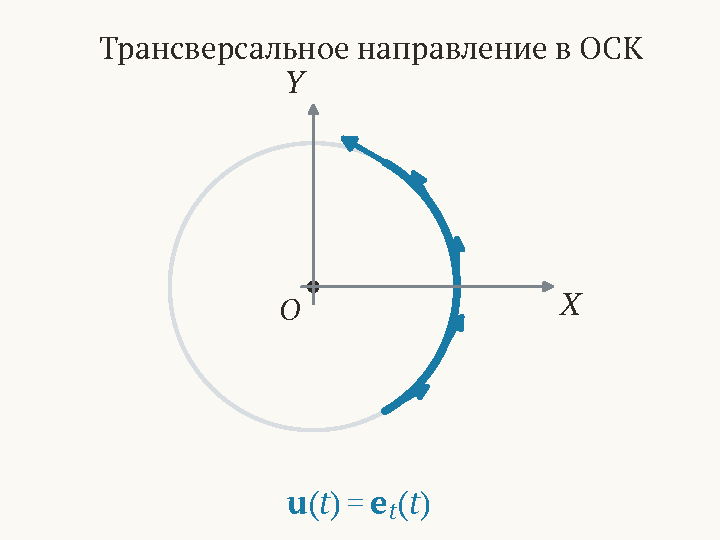
\includegraphics[width=\linewidth,height=41mm,keepaspectratio]{images/orientation-orbital-slide.pdf}
\par\smallskip
\raggedright Базис ОСК поворачивается; инерциальное направление тяги меняется.
\end{column}
\begin{column}{.49\textwidth}
\centering
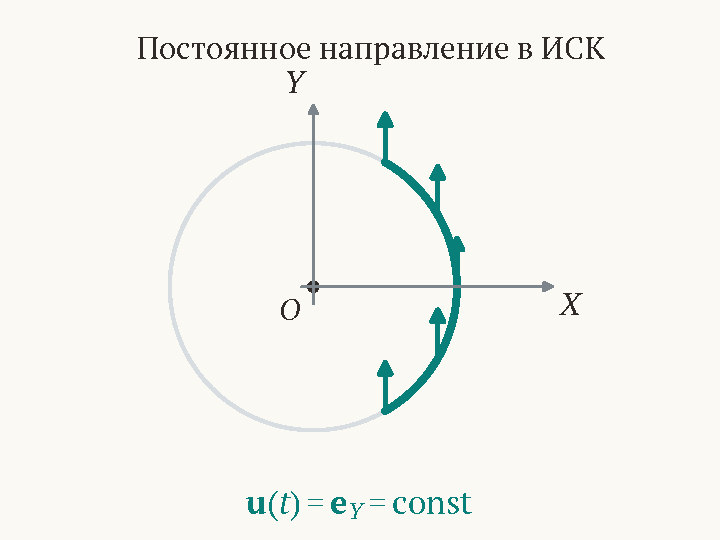
\includegraphics[width=\linewidth,height=41mm,keepaspectratio]{images/orientation-inertial-slide.pdf}
\par\smallskip
\raggedright Векторы тяги параллельны; их компоненты в текущей ОСК меняются.
\end{column}
\end{columns}
\smallskip
На круговой орбите наглядно видна разница двух законов направления тяги.
\end{frame}

\begin{frame}{Характеристическая скорость и длительность}
\relax\derivationmathspacing
\begin{columns}[T,onlytextwidth]
\begin{column}{.48\textwidth}
\textbf{Интеграл модуля ускорения}
{\eqcompact\derivationmathspacing
\[
 \Delta V=\int_{t_b}^{t_e}\|\vect a(t)\|\,\mathrm dt
         =\int_{t_b}^{t_e}\frac{F(t)}{m(t)}\,\mathrm dt,
\]
\[
 \tau=t_e-t_b,\qquad F\,\mathrm dt=-c\,\mathrm dm,
\]
\[
 \Delta V=-c\int_{m_b}^{m_e}\frac{\mathrm dm}{m}
          =c\ln\frac{m_b}{m_e},\qquad c=\mathrm{const},
\]
\[
 \boxed{m_e=m_b e^{-\Delta V/c}.}
\]
}
Расход топлива определяется $\Delta V$ и $c$; направление тяги в эту связь не входит.
\end{column}
\begin{column}{.49\textwidth}
\textbf{Постоянная тяга $F>0$}
{\eqcompact\derivationmathspacing
\[
 m(t)=m_b-\frac Fc(t-t_b),
\]
\[
 \boxed{\tau=\frac{c(m_b-m_e)}F
       =\frac{m_bc}F\left(1-e^{-\Delta V/c}\right).}
\]
\[
 \Delta V/c\ll1:\qquad\tau\simeq\frac{m_b\Delta V}F.
\]
}
Точная длительность меньше оценки с начальной массой: ускорение возрастает во время манёвра.
\par\smallskip
$b$ --- начало (begin), $e$ --- конец (end); $m_b=m(t_b)$, $m_e=m(t_e)$.
\end{column}
\end{columns}
\end{frame}

\begin{frame}{Изменение вектора скорости}
\relax\derivationmathspacing
{\eqcompact\derivationmathspacing
\[
 \vect V_e-\vect V_b=
 \int_{t_b}^{t_e}\left(-\frac{\mu\vect R}{R^3}
                    +\vect a_{\text{возм}}\right)\mathrm dt
 +\int_{t_b}^{t_e}\vect a(t)\,\mathrm dt.
\]
\[
 \left\|\int_{t_b}^{t_e}\vect a(t)\,\mathrm dt\right\|
 \le\int_{t_b}^{t_e}\|\vect a(t)\|\,\mathrm dt=\Delta V.
\]
}
\begin{columns}[T,onlytextwidth]
\begin{column}{.48\textwidth}
\textbf{Постоянное направление в ИСК}
\par\smallskip
Вклады двигателя параллельны: модуль их суммы равен $\Delta V$.
\par\smallskip
Полное $\vect V_e-\vect V_b$ включает гравитацию и возмущения.
\end{column}
\begin{column}{.49\textwidth}
\textbf{Поворот направления тяги}
\par\smallskip
Модуль векторной суммы вкладов двигателя может быть меньше $\Delta V$.
\par\smallskip
$\Delta V$ задаёт расход топлива. Конечная скорость и орбита зависят от всего движения.
\end{column}
\end{columns}
\end{frame}

\begin{frame}{Энергия и орбитальный момент}
\relax\derivationmathspacing
{\eqcompact\derivationmathspacing
\[
 \mathcal E=\frac{V^2}{2}-\frac\mu R,\qquad
 \vect h=\vect R\times\vect V,\qquad
 a=-\frac\mu{2\mathcal E},\qquad
 e^2=1+\frac{2\mathcal E h^2}{\mu^2}.
\]
}
\begin{columns}[T,onlytextwidth]
\begin{column}{.48\textwidth}
\textbf{Производная энергии}
{\eqcompact\derivationmathspacing
\[
 \dot{\mathcal E}
 =\vect V\cdot\vect a_{\text{возм}}+\frac Fm\vect V\cdot\vect u.
\]
}
Центральное ускорение сокращается с производной потенциала.
\par\smallskip
Вклад тяги зависит от скорости и угла между скоростью и тягой.
\end{column}
\begin{column}{.49\textwidth}
\textbf{Производная момента}
{\eqcompact\derivationmathspacing
\[
 \dot{\vect h}
 =\vect R\times\vect a_{\text{возм}}+\frac Fm\vect R\times\vect u.
\]
}
Момент центрального ускорения равен нулю.
\par\smallskip
Вклад тяги зависит от радиус-вектора и направления тяги.
\end{column}
\end{columns}
\smallskip
Обе производные интегрируются вдоль траектории: одно $\Delta V$ может давать разные $a$ и $e$.
\end{frame}

\begin{frame}{Выбор места манёвра}
\relax\derivationmathspacing
Для импульса точные изменения энергии и момента:
{\eqcompact\derivationmathspacing
\[
 \Delta\mathcal E=\vect V^-\cdot\Delta\vect V
                   +\frac{\|\Delta\vect V\|^2}{2},\qquad
 \Delta\vect h=\vect R\times\Delta\vect V.
\]
}
\begin{columns}[T,onlytextwidth]
\begin{column}{.48\textwidth}
\textbf{Увеличение энергии}
\par\smallskip
В данной точке при фиксированном $\Delta V$ выгоден импульс вдоль скорости:
{\eqcompact\derivationmathspacing
\[
 \Delta\mathcal E=V\Delta V+\frac{\Delta V^2}{2}.
\]
}
На одной эллиптической орбите $V$ максимально в перицентре: там наибольшее увеличение энергии.
\end{column}
\begin{column}{.49\textwidth}
\textbf{Увеличение модуля момента}
\par\smallskip
Для трансверсального импульса по движению $\Delta\vect h$ параллелен $\vect h$:
{\eqcompact\derivationmathspacing
\[
 \Delta h=R\Delta V.
\]
}
Наибольшее плечо $R$ --- в апоцентре. При том же $\Delta V$ увеличение $h$ там максимально.
\end{column}
\end{columns}
\smallskip
Требования к энергии и моменту выделяют разные точки орбиты.
\end{frame}

\begin{frame}{Начало и центр манёвра}
\relax\derivationmathspacing
{\eqcompact\derivationmathspacing
\[
 \tau=t_e-t_b,\qquad t_c=\frac{t_b+t_e}{2},\qquad
 t_{\mathrm{imp}}\text{ --- момент исходного импульса}.
\]
}
\begin{columns}[T,onlytextwidth]
\begin{column}{.48\textwidth}
\textbf{Центрирование относительно импульса}
{\eqcompact\derivationmathspacing
\[
 t_c=t_{\mathrm{imp}},\qquad
 \boxed{\begin{aligned}
 t_b&=t_{\mathrm{imp}}-\tau/2,\\
 t_e&=t_{\mathrm{imp}}+\tau/2.
 \end{aligned}}
\]
}
Воздействие распределено до и после момента исходного импульса.
\end{column}
\begin{column}{.49\textwidth}
\textbf{Начало в момент импульса}
{\eqcompact\derivationmathspacing
\[
 \boxed{\begin{aligned}
 t_b&=t_{\mathrm{imp}},\\
 t_e&=t_{\mathrm{imp}}+\tau,
 \end{aligned}}\qquad
 t_c=t_{\mathrm{imp}}+\frac\tau2.
\]
}
Весь манёвр смещён вперёд; его центр сдвинут на $\tau/2$.
\end{column}
\end{columns}
\smallskip
Варианты сравниваются при одном $t_f$: меняются положение КА во время тяги и длительность пассивного движения после неё.
\end{frame}

\begin{frame}{Угловая протяжённость манёвра}
\relax\derivationmathspacing
На опорной кеплеровской орбите $\dot\nu=h/R^2$:
{\eqcompact\derivationmathspacing
\[
 \boxed{\theta=\nu(t_e)-\nu(t_b)
       =\int_{t_b}^{t_e}\frac{h}{R(t)^2}\,\mathrm dt,}
 \qquad h=\|\vect R\times\vect V\|.
\]
}
\begin{columns}[T,onlytextwidth]
\begin{column}{.48\textwidth}
\textbf{Эллиптическая орбита}
\begin{itemize}
\setlength{\itemsep}{3pt}
\item Аномалии не приводятся к одному обороту.
\item При одной $\tau$ угол $\theta$ больше у перицентра и меньше у апоцентра.
\item Отношения длительности к периоду недостаточно для оценки локальности.
\end{itemize}
\end{column}
\begin{column}{.49\textwidth}
\textbf{Два условия приближения}
\begin{itemize}
\setlength{\itemsep}{3pt}
\item Малость $\Delta V/V$ и изменений элементов позволяет линеаризацию.
\item Малое изменение чувствительности за время тяги позволяет замену импульсом.
\end{itemize}
\end{column}
\end{columns}
\end{frame}

\begin{frame}{Матрица манёвра и конечное состояние}
\relax\derivationmathspacing
{\eqcompact\derivationmathspacing
\[
 M(t)=\Phi(t_f,t)B(t),\qquad
 \boxed{\delta\vect y_f=\int_{t_b}^{t_e}M(t)\vect a(t)\,\mathrm dt.}
\]
}
\begin{columns}[T,onlytextwidth]
\begin{column}{.48\textwidth}
\textbf{Смысл матриц}
\begin{itemize}
\setlength{\itemsep}{2pt}
\item $B(t)$ задаёт изменение переменных под действием ускорения.
\item $\Phi(t_f,t)$ переносит отклонение из $t$ в $t_f$.
\item $M(t)$ задаёт конечный результат управления.
\end{itemize}
\end{column}
\begin{column}{.49\textwidth}
\textbf{Опорная траектория}
\begin{itemize}
\setlength{\itemsep}{2pt}
\item Матрицы считаются вдоль опорной траектории.
\item Для пассивной орбиты $\vect a$ --- добавляемое ускорение.
\item Для движения с тягой --- малое изменение ускорения.
\end{itemize}
\end{column}
\end{columns}
\smallskip
Компоненты $\vect a$ и столбцы $B$ --- в одной системе; поворот ОСК включён в $B(t)$.
\end{frame}

\begin{frame}{Почему помогает центрирование}
\relax\derivationmathspacing
Постоянный столбец ускорения $\vect a=\Delta\vect V/\tau$; $s=t-t_c$.
{\eqcompact\derivationmathspacing
\[
 \delta\vect y_f=\overline M\Delta\vect V,\qquad
 \overline M=\frac1\tau\int_{-\tau/2}^{\tau/2}M(t_c+s)\,\mathrm ds.
\]
\[
 M(t_c+s)=M(t_c)+s\dot M(t_c)+\frac{s^2}{2}\ddot M(t_c)
                 +\frac{s^3}{6}M^{(3)}(t_c)+O(s^4).
\]
}
{\eqcompact\derivationmathspacing
\[
 \int_{-\tau/2}^{\tau/2}s\,\mathrm ds=
 \int_{-\tau/2}^{\tau/2}s^3\,\mathrm ds=0,\qquad
 \int_{-\tau/2}^{\tau/2}s^2\,\mathrm ds=\frac{\tau^3}{12}.
\]
}
{\eqcompact\derivationmathspacing
\[
 \boxed{\overline M=M(t_c)+\frac{\tau^2}{24}\ddot M(t_c)+O(\tau^4).}
\]
}
Нечётные члены сокращаются. Импульс в центре дал бы $M(t_c)\Delta\vect V$; разность матриц начинается с члена порядка $\tau^2$.
\end{frame}

\begin{frame}{Размещение и профиль ускорения}
\relax\derivationmathspacing
При начале манёвра в момент импульса интервал несимметричен:
{\eqcompact\derivationmathspacing
\[
 \frac1\tau\int_{t_{\mathrm{imp}}}^{t_{\mathrm{imp}}+\tau}M(t)\,\mathrm dt
 =M(t_{\mathrm{imp}})+\frac\tau2\dot M(t_{\mathrm{imp}})
 +\frac{\tau^2}{6}\ddot M(t_{\mathrm{imp}})+O(\tau^3).
\]
}
\begin{columns}[T,onlytextwidth]
\begin{column}{.48\textwidth}
\textbf{Постоянное ускорение}
\par\smallskip
При начале в $t_{\mathrm{imp}}$ сохраняется член $\tau\dot M/2$.
\par\smallskip
При центрировании ошибка усреднения начинается со второго порядка по длительности вместо первого.
\end{column}
\begin{column}{.49\textwidth}
\textbf{Переменный модуль}
\par
Направление в выбранной системе компонент неизменно:
{\eqcompact\derivationmathspacing
\[
 w(t)=\frac{\|\vect a(t)\|}{\Delta V},\qquad
 \overline t=\int_{t_b}^{t_e}t\,w(t)\,\mathrm dt.
\]
}
{\eqcompact\derivationmathspacing
\[
 \dot M(t_c)(\overline t-t_c)\Delta\vect V.
\]
}
Симметрия профиля даёт $\overline t=t_c$. При постоянной тяге ускорение растёт: симметрии границ недостаточно.
\end{column}
\end{columns}
\end{frame}

% Глава 3 методички: вспомогательный пример на круговой опорной орбите.
\begin{frame}{Пример около круговой орбиты}
\relax
\derivationmathspacing
{\eqcompact\derivationmathspacing
\[
 V_0=\sqrt{\frac\mu{r_0}},\qquad
 n_0=\sqrt{\frac\mu{r_0^3}},\qquad
 \varphi=n_0(t-t_c),\qquad
 \theta=n_0\tau,\qquad A=\frac{\Delta V}{\tau}.
\]
}
\begin{columns}[T,onlytextwidth]
\begin{column}{.45\textwidth}
\textbf{Изменение энергии и формы}
{\eqcompact\derivationmathspacing
\[
 \dot{\mathcal E}=V_0T,\qquad
 \dot a=\frac{2r_0}{V_0}T,
\]
\[
 \dot{\vect e}=\frac{2T\vect e_r-S\vect e_t}{V_0}.
\]
\[
 \begin{aligned}
 \vect e_r&=(\cos\varphi,\sin\varphi)^\top,\\
 \vect e_t&=(-\sin\varphi,\cos\varphi)^\top.
 \end{aligned}
\]
}
\justifying
Неподвижные оси: $X$ --- радиус в $t_c$;
$Y$ --- скорость в $t_c$. Начальный $\vect e=0$.
\end{column}
\begin{column}{.52\textwidth}
\textbf{Интегралы первого порядка}
{\eqcompact\derivationmathspacing
\[
\begin{aligned}
 \delta a&=\frac{2r_0}{V_0}\int_{t_b}^{t_e}T\,\mathrm d t,\\[1pt]
 \delta e_x&=\frac1{V_0}\int_{t_b}^{t_e}
       (S\sin\varphi+2T\cos\varphi)\,\mathrm d t,\\[1pt]
 \delta e_y&=\frac1{V_0}\int_{t_b}^{t_e}
       (-S\cos\varphi+2T\sin\varphi)\,\mathrm d t.
\end{aligned}
\]
}
\justifying
Первый порядок по $\varepsilon=\Delta V/V_0\ll1$
при фиксированном $\theta$. Малость $\theta$ не требуется.
\end{column}
\end{columns}
\end{frame}

\begin{frame}{Трансверсальное направление в ОСК}
\relax
\derivationmathspacing
{\centering
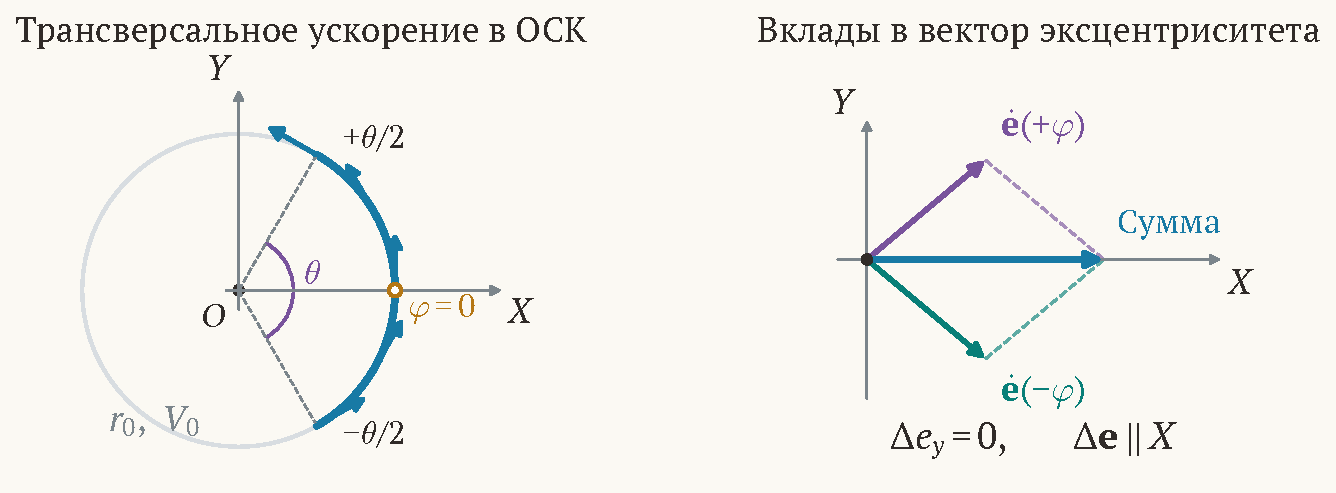
\includegraphics[width=\textwidth,height=44mm,keepaspectratio]{images/circle-orbital-slide.pdf}\par}
{\eqcompact\par\centering $\displaystyle
 S=0,\quad T=A:
 \qquad
 \delta a=\frac{2r_0\Delta V}{V_0},\qquad
 \delta e_x=\frac{2\Delta V}{V_0}\operatorname{sinc}\frac\theta2,
 \qquad\delta e_y=0.
$\par
}
\justifying
$\operatorname{sinc} x=\sin x/x$, $\operatorname{sinc}0=1$. При росте $\theta$ изменение $a$ постоянно,
а изменение $e_x$ уменьшается из-за разных направлений частных вкладов.
\end{frame}

\begin{frame}{Постоянное инерциальное направление}
\relax
\derivationmathspacing
{\eqcompact $S=A\sin\varphi$, $T=A\cos\varphi$. В центре манёвра $\vect a=A\vect e_t$.\par}
{\centering
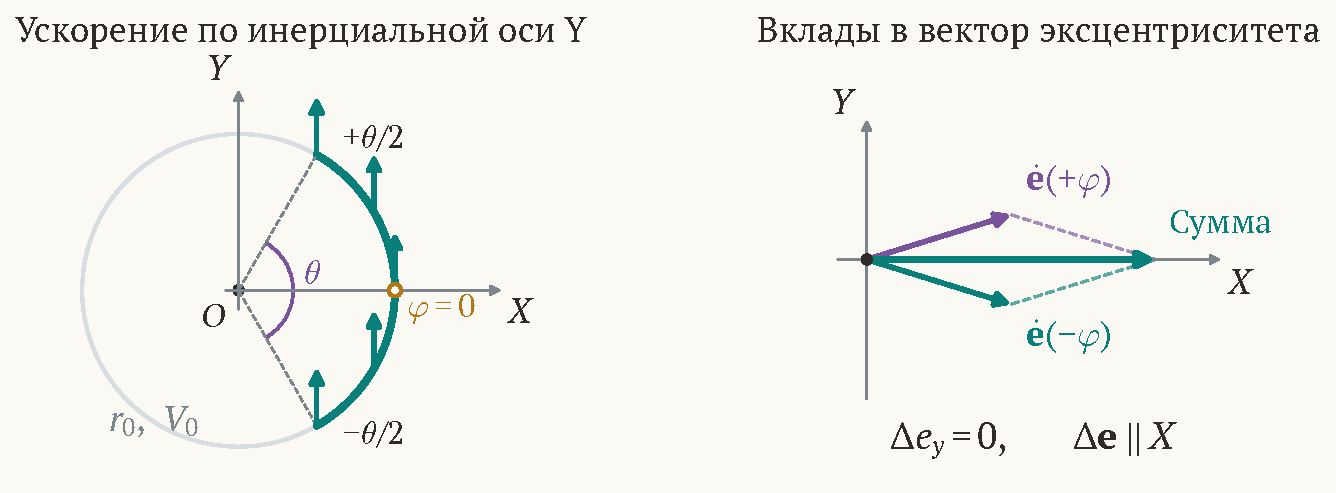
\includegraphics[width=\textwidth,height=41.5mm,keepaspectratio]{images/circle-inertial-slide.pdf}\par}
{\eqcompact\par\centering $\displaystyle
 \delta a=\frac{2r_0\Delta V}{V_0}\operatorname{sinc}\frac\theta2,\qquad
 \delta e_x=\frac{2\Delta V}{V_0}
 \left(\frac34+\frac14\operatorname{sinc}\theta\right),\qquad \delta e_y=0.
$\par
}
\justifying
Радиальная составляющая также меняет $e_x$,
а $T<A$ на краях участка уменьшает изменение $a$.
\end{frame}

\begin{frame}{Разные орбитальные результаты одного $\Delta V$}
\relax
\derivationmathspacing
{\eqcompact\par\centering $\displaystyle
 k_a=\frac{\delta a}{2r_0\Delta V/V_0},\qquad
 k_e=\frac{\delta e_x}{2\Delta V/V_0}.
$\par
}
{\centering
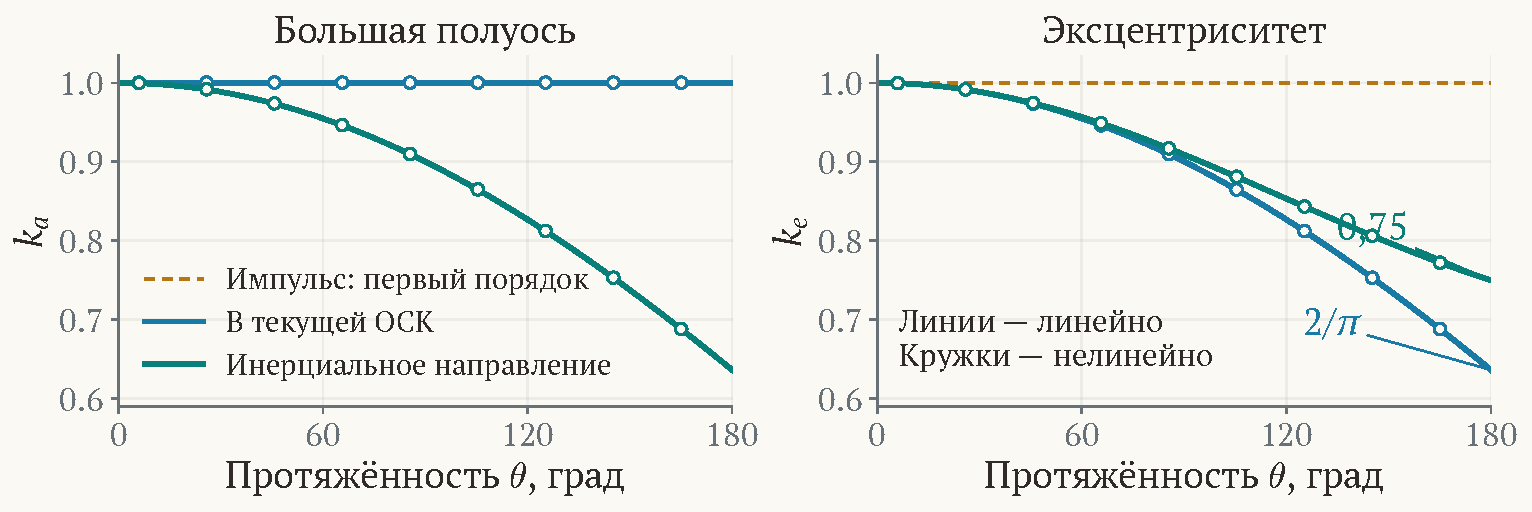
\includegraphics[width=\textwidth,height=44.5mm,keepaspectratio]{images/circular-response-slide.pdf}\par}
\justifying
Эффективность зависит от изменяемого элемента орбиты:
единого коэффициента при $\Delta V$ для всех орбитальных результатов нет.
\end{frame}

\begin{frame}{Численная проверка кругового примера}
\relax
\derivationmathspacing
{\eqcompact\par\centering $\displaystyle
 r_0=\CircRadius\ \text{км},\quad
 \Delta V=\CircDVMps\ \text{м/с},\quad
 V_0=\CircVelocity\ \text{км/с},\quad
 \frac{\Delta V}{V_0}\simeq1.33\cdot10^{-4}.
$\par
}
Период --- $\CircPeriodMinutes$ мин;
при $\theta=180^\circ$ длительность $\tau=\CircHalfOrbitMinutes$ мин.
{\centering
\eqcompact\derivationmathspacing
\renewcommand{\arraystretch}{1.16}
\begin{tabular}{@{}lrrrr@{}}
\toprule
&\multicolumn{2}{c}{$\delta a$, м}
&\multicolumn{2}{c}{$e_x\cdot10^4$}\\
Направление&Линейно&Нелинейно&Линейно&Нелинейно\\\midrule
В текущей ОСК&1855{,}274&1855{,}743&1{,}687292&1{,}687572\\
В инерциальной системе&1181{,}104&1181{,}403&1{,}987794&1{,}987878\\
\bottomrule
\end{tabular}\par
}
\par\vspace{3mm}
\begin{columns}[T,onlytextwidth]
\begin{column}{.47\textwidth}
\textbf{Нелинейный расчёт}\par
\justifying
Начальное состояние в $t_b$ --- на опорной орбите.
Центральное поле, $A=\Delta V/\tau$.
Текущая ОСК определяется по состоянию КА.
\end{column}
\begin{column}{.50\textwidth}
\textbf{Разность на $1$--$180^\circ$}
{\eqcompact\derivationmathspacing
\[
 |\delta a_{\text{нелин}}-\delta a_{\text{лин}}|<0.615\ \text{м},
\]
\[
 r_0\lVert\vect e_{\text{нелин}}-\vect e_{\text{лин}}\rVert<0.197\ \text{м}.
\]
}
\justifying
Ужесточение допусков и уменьшение шага:
изменение менее $3\cdot10^{-8}$ м.
\end{column}
\end{columns}
\end{frame}


% Главы 4--6 текущей методички finite-maneuvers.tex.
% Макросы и оформление повторяют 7/7.tex; самостоятельной преамбулы нет.

\begin{frame}{Распределение манёвра между витками}
\relax\derivationmathspacing
\begin{columns}[T,onlytextwidth]
\begin{column}{.45\textwidth}
\textbf{Веса характеристической скорости}
{\eqcompact\derivationmathspacing
\[
 \Delta V_j=w_j\Delta V_{\text{гр}},\qquad
 w_j\geqslant0,\qquad \sum_{j=1}^N w_j=1.
\]
}
Один импульс заменяется группой из $N$ манёвров.
Положения и направления тяги назначаются отдельно.
\par\smallskip
Для прогноза нужны начальное состояние и масса,
$t_{b,j}$, $\tau_j$, тяга, $I_{\mathrm{sp}}$, направление тяги,
модель возмущений и конечная эпоха.
\end{column}
\begin{column}{.52\textwidth}
\textbf{Масса и длительность при постоянных $F,c$}
{\eqcompact\derivationmathspacing
\[
 m_{e,j}=m_{b,j}\exp\!\left(-\frac{w_j\Delta V_{\text{гр}}}{c}\right),
\]
\[
 \tau_j=\frac{c\,m_{b,j}}{F}
 \left[1-\exp\!\left(-\frac{w_j\Delta V_{\text{гр}}}{c}\right)\right].
\]
}
На паузах $m_{b,j+1}=m_{e,j}$.
Равные $\Delta V_j$ дают уменьшающиеся длительности.
\par\smallskip
При равном времени расход массы одинаков, а $\Delta V_j$ возрастают.
\end{column}
\end{columns}
\end{frame}

\begin{frame}{Перенос манёвра на следующий виток}
\relax\derivationmathspacing
\begin{columns}[T,onlytextwidth]
\begin{column}{.48\textwidth}
\textbf{Положение манёвра}
\begin{itemize}
\setlength{\itemsep}{5pt}
\item Около перицентров последующих орбит.
\item В прежнем инерциальном направлении радиуса.
\end{itemize}
\smallskip
Способы совпадают, пока линия апсид сохраняет положение.
При её повороте положения на орбите различаются.
\end{column}
\begin{column}{.49\textwidth}
\textbf{Направление тяги}
\begin{itemize}
\setlength{\itemsep}{5pt}
\item Инерциальное направление исходного импульса.
\item Его компоненты в ОСК центра следующего манёвра.
\end{itemize}
\smallskip
Выбор зависит от назначения манёвра: изменения
размера, формы или плоскости орбиты.
\end{column}
\end{columns}
\par\medskip
Одинаковая сумма $\Delta V_j$ при разных положениях
и направлениях даёт разные орбиты.
\end{frame}

\begin{frame}{Ошибки исполнения манёвров}
\relax\derivationmathspacing
\begin{columns}[T,onlytextwidth]
\begin{column}{.48\textwidth}
\textbf{Относительная и абсолютная ошибки}
{\eqcompact\derivationmathspacing
\[
 \delta_j=
 \frac{\Delta V_{j,\text{факт}}-\Delta V_{j,\text{план}}}
      {\Delta V_{j,\text{план}}},
\]
\[
 \Delta V_{j,\text{факт}}=(1+\delta_j)\Delta V_{j,\text{план}}.
\]
}
При $\delta_j=0{,}01$ превышение составляет $1\%$.
Абсолютная ошибка: $\delta_j\Delta V_{j,\text{план}}$.
\par\smallskip
У меньшего манёвра она меньше при одинаковой относительной ошибке.
При одинаковой угловой ошибке направления меньше и векторная ошибка.
\end{column}
\begin{column}{.49\textwidth}
\textbf{Общая систематическая ошибка}
{\eqcompact\derivationmathspacing
\[
 \begin{aligned}
 \sum_j\Delta V_{j,\text{факт}}
 &=(1+\delta_{\text{сист}})
      \sum_j\Delta V_{j,\text{план}}\\
 &=(1+\delta_{\text{сист}})\Delta V_{\text{гр}}.
 \end{aligned}
\]
}
Результат не зависит от выбранных весов.
Дробление само по себе такую ошибку не устраняет.
\par\smallskip
Последовательность полезна, если по первым манёврам можно оценить
отклонение, уточнить модель двигателя и изменить последующие манёвры.
\end{column}
\end{columns}
\end{frame}

\begin{frame}{Равные и убывающие веса}
\relax\derivationmathspacing
\begin{columns}[T,onlytextwidth]
\begin{column}{.48\textwidth}
\textbf{Равные веса}
{\eqcompact\derivationmathspacing
\[
 \max_j\Delta V_j\geqslant
 \frac1N\sum_j\Delta V_j=\frac{\Delta V_{\text{гр}}}{N}.
\]
}
Равные веса $w_j=1/N$ минимизируют наибольшую $\Delta V_j$
при заданных сумме и числе манёвров.
\par\smallskip
Это помогает ограничить воздействие вдали от выбранного положения.
Длительности зависят ещё от массы, пройденные углы --- от движения по орбите.
\end{column}
\begin{column}{.49\textwidth}
\textbf{Убывающие веса}
\par\smallskip
Веса пропорциональны $1,k,k^2,\ldots,k^{N-1}$,
$0<k<1$; сумма нормируется к единице.
\par\smallskip
Большая часть изменения выполняется раньше.
У малого последнего манёвра меньше абсолютная ошибка
при той же относительной.
\par\smallskip
Для коррекции нужен запас величины и допустимого направления.
Оставшиеся манёвры пересчитывают по достигнутой орбите.
\end{column}
\end{columns}
\end{frame}

\begin{frame}{Коррекция последующими манёврами}
\relax\derivationmathspacing
{\eqcompact\derivationmathspacing
\[
 \Delta\vect V_1\ \longrightarrow\ \Delta\vect V_1+\vect\varepsilon
 \quad\Rightarrow\quad
 \Delta\vect V_{\text{ост}}\ \longrightarrow\
 \Delta\vect V_{\text{ост}}-\vect\varepsilon.
\]
}
{\centering
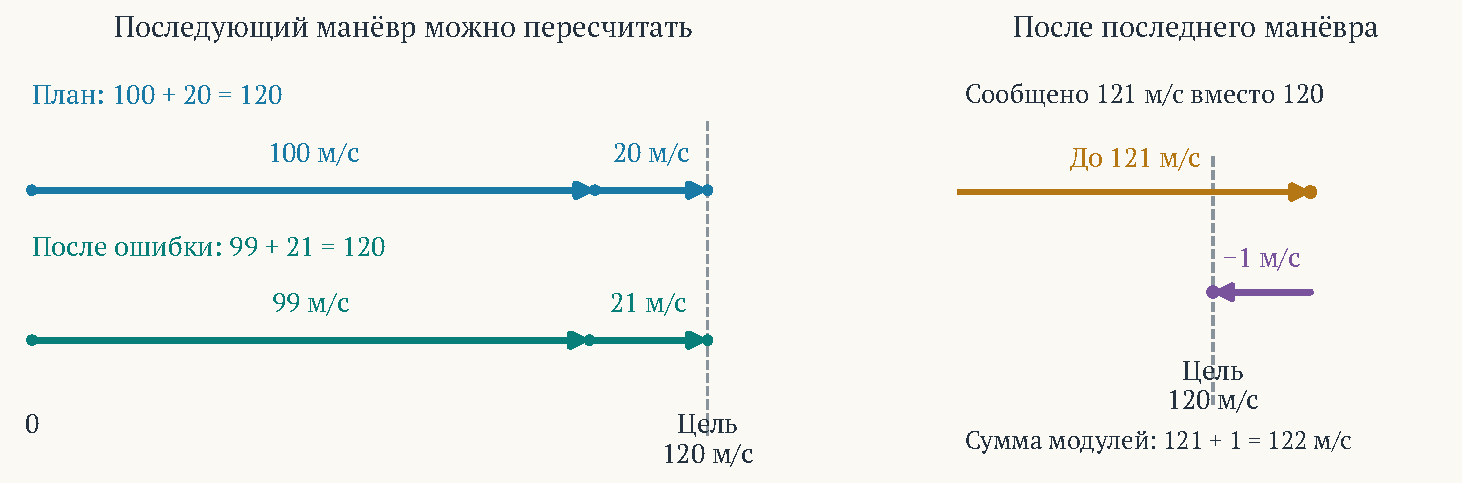
\includegraphics[width=\textwidth,height=43mm,keepaspectratio]{images/error-compensation-slide.pdf}\par}
Схема: одна точка и общая система координат. На орбите оставшиеся
манёвры пересчитываются из фактически достигнутого состояния.
\end{frame}

\begin{frame}{Последовательный прогноз}
\relax\derivationmathspacing
{\centering
\begin{tikzpicture}[x=.94cm,y=.76cm,>=Latex,font=\fontsize{9.5}{11.5}\selectfont]
\draw[->,courseink] (0,0)--(15,0) node[right] {$t$};
\foreach \l/\r/\name in {2/4/1,7/8.4/2,11.7/12.5/3}{
 \fill[courseaccent!18] (\l,.15) rectangle (\r,1.15);
 \draw[courseaccent,thick] (\l,.15)--(\l,1.15)--(\r,1.15)--(\r,.15);
 \node[courseaccent] at ({(\l+\r)/2},1.43) {манёвр \name};
 \draw[densely dashed,coursemuted] (\l,0)--(\l,1.2);
 \draw[densely dashed,coursemuted] (\r,0)--(\r,1.2);
}
\node[coursemuted] at (1,.55) {прогноз};
\node[coursemuted] at (5.5,.55) {пауза};
\node[coursemuted] at (10,.55) {пауза};
\node[coursemuted] at (13.7,.55) {прогноз};
\node[below] at (0,0) {$t_0$};
\node[below] at (2,0) {$t_{b,1}$};
\node[below] at (4,0) {$t_{e,1}$};
\node[below] at (14.7,0) {$t_f$};
\draw[<->,courseaccent] (2,-.7)--node[below] {$\tau_1$}(4,-.7);
\draw[<->,coursemuted] (4,-.7)--node[below] {$\Delta t_1$}(7,-.7);
\end{tikzpicture}\par}
\begin{columns}[T,onlytextwidth]
\begin{column}{.48\textwidth}
\begin{enumerate}
\setlength{\itemsep}{4pt}
\item Пассивное движение до $t_{b,1}$.
\item Движение с тягой до $t_{e,1}=t_{b,1}+\tau_1$.
\item Полученные элементы и масса --- начальные данные
следующего участка.
\end{enumerate}
\end{column}
\begin{column}{.49\textwidth}
\begin{enumerate}
\setcounter{enumi}{3}
\setlength{\itemsep}{4pt}
\item Повторить пассивный участок и манёвр
для всей последовательности.
\item После последнего манёвра продолжить прогноз до $t_f$
и проверить конечные условия.
\end{enumerate}
\end{column}
\end{columns}
\end{frame}

\begin{frame}{Возмущения меняют геометрию манёвра}
\relax\derivationmathspacing
\begin{columns}[T,onlytextwidth]
\begin{column}{.51\textwidth}
\centering
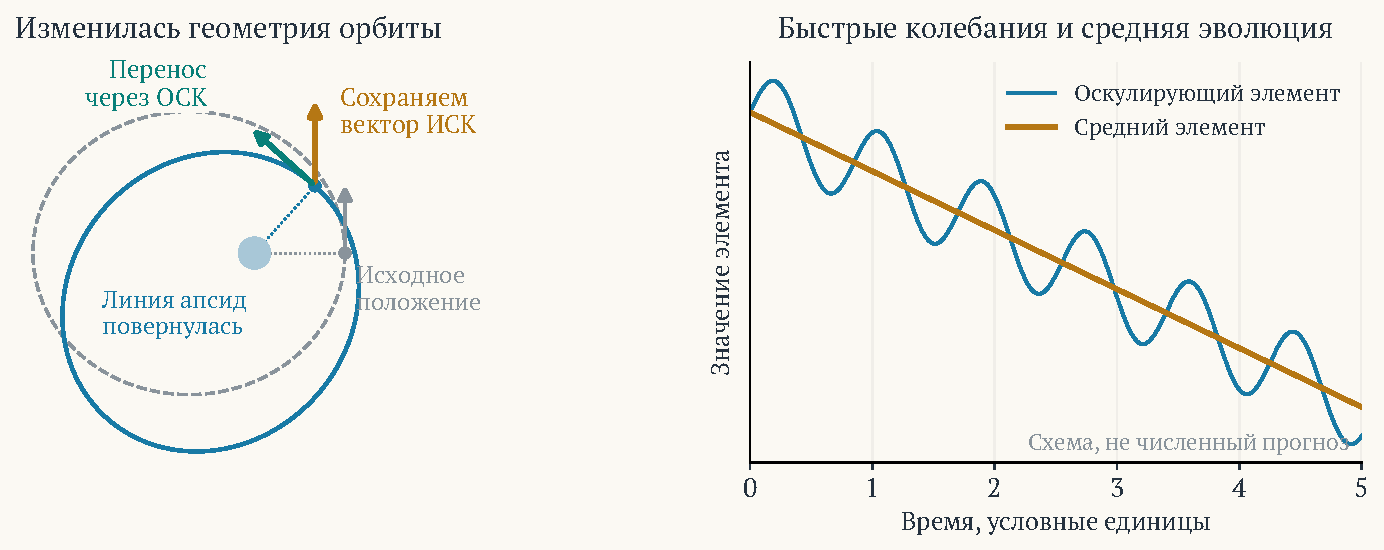
\includegraphics[width=\linewidth,height=56mm,keepaspectratio,trim=0bp 0bp 374bp 0bp,clip]{images/perturbed-geometry-slide.pdf}
\end{column}
\begin{column}{.46\textwidth}
$J_2$ вызывает прецессию линии узлов и линии апсид.
\par\smallskip
Для изменения энергии около перицентра положение манёвра
выбирается по новой орбите.
\par\smallskip
Поворот плоскости меняет компоненты постоянного вектора ИСК
в местной ОСК.
\par\smallskip
Возмущения учитываются на активных и пассивных участках.
\end{column}
\end{columns}
\end{frame}

\begin{frame}{Перенос направления между манёврами}
\relax\derivationmathspacing
Базис ОСК в центре $j$-го манёвра:
{\eqcompact\derivationmathspacing
\[
 Q_j=\begin{pmatrix}\vect e_{r,j}&\vect e_{t,j}&\vect e_{n,j}\end{pmatrix},
 \qquad \vect d=Q_1^\top\vect u_1.
\]
}
\begin{columns}[T,onlytextwidth]
\begin{column}{.48\textwidth}
\textbf{Сохраняем инерциальное направление}
{\eqcompact\derivationmathspacing
\[
 \vect u_j=\vect u_1.
\]
}
КА воспроизводит один вектор в пространстве.
Его компоненты в изменившейся ОСК, вообще говоря, другие.
\end{column}
\begin{column}{.49\textwidth}
\textbf{Сохраняем компоненты в ОСК центра}
{\eqcompact\derivationmathspacing
\[
 \vect u_j=Q_j\vect d.
\]
}
По новому прогнозу положения и скорости строится $Q_j$
и новое направление в ИСК.
\end{column}
\end{columns}
\par\medskip
Во время манёвра $\vect u_j$ можно сохранять постоянным в ИСК.
Непрерывная ориентация по текущей ОСК --- отдельный закон управления.
\end{frame}

\begin{frame}{Оскулирующие и средние элементы}
\relax\derivationmathspacing
\begin{columns}[T,onlytextwidth]
\begin{column}{.50\textwidth}
\centering
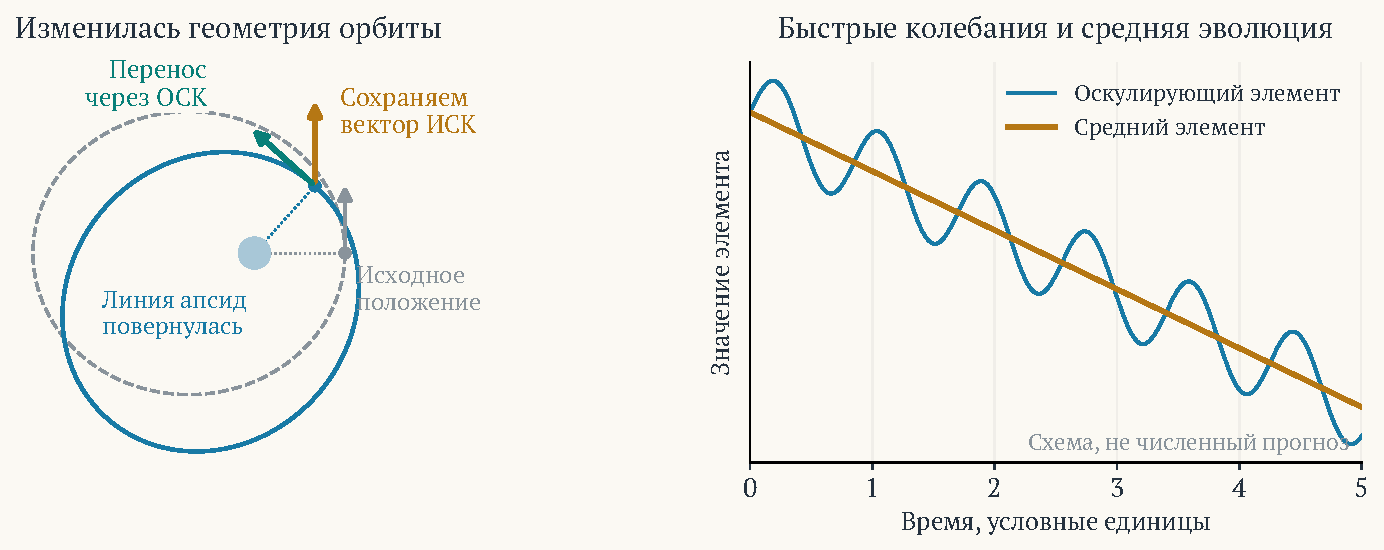
\includegraphics[width=\linewidth,height=55mm,keepaspectratio,trim=333bp 0bp 0bp 0bp,clip]{images/perturbed-geometry-slide.pdf}
\end{column}
\begin{column}{.47\textwidth}
\textbf{Оскулирующая орбита}: те же текущие положение и скорость КА.
\par\smallskip
\textbf{Средние элементы}: исключены выбранные периодические составляющие.
\par\smallskip
Среднюю цель и результат получают по одной модели усреднения.
\par\smallskip
Оскулирующие элементы сравнивают в общей эпохе $t_f$.
\end{column}
\end{columns}
\end{frame}

\begin{frame}{Невязка конечных условий}
\relax\derivationmathspacing
{\eqcompact\derivationmathspacing
\[
 \boxed{\vect F(\vect q)=\vect y(t_f;\vect q)-\vect y_{\text{цель}}=0.}
\]
}
\begin{columns}[T,onlytextwidth]
\begin{column}{.48\textwidth}
\textbf{Свободные параметры $\vect q$}
\begin{itemize}
\setlength{\itemsep}{5pt}
\item Длительности манёвров.
\item Компоненты направлений тяги.
\item Положения центров.
\item Характеристические скорости групп.
\end{itemize}
Исходное состояние и конечная эпоха фиксированы.
\end{column}
\begin{column}{.49\textwidth}
\textbf{Конечные величины $\vect y$}
Включают именно те параметры конечной орбиты или состояния,
которые требуется сформировать.
\par\smallskip
Для каждого $\vect q$ рассчитывается вся траектория до $t_f$.
\par\smallskip
Компоненты невязки приводятся к безразмерной форме;
нормировка задаётся вместе с задачей.
\end{column}
\end{columns}
\end{frame}

\begin{frame}{Как параметры меняют конечную орбиту}
\relax\derivationmathspacing
Линеаризация по малой поправке $\delta\vect q$:
{\eqcompact\derivationmathspacing
\[
 \vect F(\vect q+\delta\vect q)\simeq
 \vect F(\vect q)+\frac{\partial\vect F}{\partial\vect q}\,\delta\vect q.
\]
}
Каждый столбец --- влияние одного параметра на все конечные невязки.
\par\smallskip
Например, $q_1=\tau_1$. Два полных прогноза с $\tau_1+h_1$ и $\tau_1-h_1$:
{\eqcompact\derivationmathspacing
\[
 \frac{\partial\vect F}{\partial\tau_1}\simeq
 \frac{\vect F(\tau_1+h_1,q_2,\ldots)
      -\vect F(\tau_1-h_1,q_2,\ldots)}{2h_1}.
\]
}
\begin{columns}[T,onlytextwidth]
\begin{column}{.48\textwidth}
Остальные столбцы: меняется по одному свободному параметру.
\end{column}
\begin{column}{.49\textwidth}
Шаг $h_k$: различимое изменение результата при достаточно
малой поправке для местной производной.
\end{column}
\end{columns}
\par\smallskip
Каждое изменение затрагивает последующие участки:
повторяется весь расчёт до $t_f$.
\end{frame}

\begin{frame}{Пристрелка с ньютоновским уточнением}
\relax\derivationmathspacing
\begin{columns}[T,onlytextwidth]
\begin{column}{.48\textwidth}
\textbf{Поправка и обновление параметров}
{\eqcompact\derivationmathspacing
\[
 \frac{\partial\vect F}{\partial\vect q}\,\delta\vect q=-\vect F(\vect q),
\]
\[
 \vect q_{\text{нов}}=\vect q+\alpha\,\delta\vect q,
 \qquad 0<\alpha\leqslant1.
\]
}
Квадратная невырожденная система даёт единственную поправку.
\par\smallskip
При избытке параметров --- поправка наименьшей нормы
в заданных единицах.
\end{column}
\begin{column}{.49\textwidth}
\textbf{Повторный нелинейный прогноз}
\begin{enumerate}
\setlength{\itemsep}{2pt}
\item Проверить полный шаг $\alpha=1$;
если невязка растёт, уменьшить шаг.
\item Пересчитать траекторию и невязку.
\item При необходимости повторить расчёт производных и поправки.
\end{enumerate}
{\eqcompact\derivationmathspacing
\[
 \boxed{\|\vect F(\vect q)\|\leqslant\varepsilon.}
\]
}
Допуск задан для безразмерной невязки.
\end{column}
\end{columns}
\par\smallskip
Малая невязка подтверждает конечные требования.
Минимум $\Delta V$ требует отдельного критерия.
\end{frame}


% Глава 7 методички 8/finite-maneuvers.tex. Только данные сохранённого расчёта.
\begin{frame}{Переход между эллиптическими орбитами}
\relax
\derivationmathspacing
\begin{columns}[T,onlytextwidth]
\begin{column}{.51\textwidth}
{\eqcompact
\centering
\renewcommand{\arraystretch}{1.12}
\begin{tabular}{@{}lrr@{}}
\toprule
Элемент & Начальная & Целевая\\\midrule
$a$, км & $18\,500$ & $42\,164$\\
$e$ & $23/37$ & $0{,}05$\\
$i$ & $7^\circ$ & $3^\circ$\\
$\Omega$ & $30^\circ$ & $30^\circ$\\
$\omega$ & $0^\circ$ & $0^\circ$\\
$\nu$ & $0^\circ$ & Свободная\\
\bottomrule
\end{tabular}\par
}
\smallskip
Начальные радиусы перигея и апогея --- $7000$ и $30\,000$ км.
\end{column}
\begin{column}{.46\textwidth}
\textbf{Аппарат и конечная эпоха}\par\smallskip
Начальная масса $2000$ кг, сухая --- $1075$ кг.
\[
\begin{gathered}
 F=450\ \text{Н},\quad I_{\rm sp}=300\ \text{с},\\
 t_f-t_0=10\ \text{суток}.
\end{gathered}
\]
Целевая орбита:
\[
\begin{aligned}
 r_{p,f}&=a_f(1-e_f)=40\,055{,}8\ \text{км},\\
 r_{a,f}&=a_f(1+e_f)=44\,272{,}2\ \text{км}.
\end{aligned}
\]
\justifying
Все пять конечных элементов задаются в общей эпохе $t_f$.
Положение КА вдоль целевой орбиты свободно.
\end{column}
\end{columns}
\end{frame}

\begin{frame}{Конечные условия в кеплеровых элементах}
\relax
\derivationmathspacing
\begin{columns}[T,onlytextwidth]
\begin{column}{.48\textwidth}
\textbf{Интегрируемое состояние}
\[
 \vect z=(a,e,i,\Omega,\omega,\nu,m)^\top.
\]
{\eqcompact\derivationmathspacing
\[
 \vect F(\vect q)=
 \begin{pmatrix}
 (a(t_f;\vect q)-a_f)/a_i\\
 e(t_f;\vect q)-e_f\\
 i(t_f;\vect q)-i_f\\
 \Delta\Omega(t_f;\vect q)\\
 \Delta\omega(t_f;\vect q)
 \end{pmatrix},
\]
\[
 a_i=18\,500\ \text{км}.
\]
}
\[
 \boxed{\lVert\vect F(\vect q)\rVert_2\leqslant\varepsilon,
 \qquad\varepsilon=10^{-8}.}
\]
\end{column}
\begin{column}{.49\textwidth}
\begin{itemize}
\setlength{\itemsep}{5pt}
\item $\Delta\Omega=\Omega-\Omega_f$, $\Delta\omega=\omega-\omega_f$;
разности приводятся к $[-\pi,\pi)$.
\item В вычислениях углы выражаются в радианах, длины --- в километрах,
время --- в секундах.
\item Элементы отсчитываются от экватора Земли; её ось симметрии фиксирована.
\item Один критерий используется при сравнении моделей,
пристрелке и повторном прогнозе.
\end{itemize}
\end{column}
\end{columns}
\end{frame}

\begin{frame}{Прогноз в кеплеровых элементах}
\relax
\derivationmathspacing
{\eqcompact\derivationmathspacing
\[
 p=a(1-e^2),\qquad h=\sqrt{\mu p},\qquad
 r=\frac p{1+e\cos\nu},\qquad u=\omega+\nu.
\]
}
\begin{columns}[T,onlytextwidth]
\begin{column}{.48\textwidth}
{\eqcompact\derivationmathspacing
\[
\begin{aligned}
 \dot a&=\frac{2a^2}{h}
 \left(e\sin\nu\,S_\Sigma+\frac pr T_\Sigma\right),\\
 \dot e&=\frac1h\bigl[p\sin\nu\,S_\Sigma\\[-2pt]
 &\hspace{7mm}+\bigl((p+r)\cos\nu+re\bigr)T_\Sigma\bigr],\\
 \dot i&=\frac{r\cos u}{h}W_\Sigma,\\
 \dot\Omega&=\frac{r\sin u}{h\sin i}W_\Sigma.
\end{aligned}
\]
}
\end{column}
\begin{column}{.49\textwidth}
{\eqcompact\derivationmathspacing
\[
\begin{aligned}
 \dot\omega={}&\frac{-p\cos\nu\,S_\Sigma+(p+r)\sin\nu\,T_\Sigma}{he}\\
 &-\frac{r\sin u\cos i}{h\sin i}W_\Sigma,\\
 \dot\nu={}&\frac h{r^2}
 +\frac{p\cos\nu\,S_\Sigma-(p+r)\sin\nu\,T_\Sigma}{he},\\
 \dot m={}&-\frac Fc,\qquad c=g_0I_{\rm sp}.
\end{aligned}
\]
}
\justifying
Истинная аномалия непрерывна, без приведения к одному обороту.
\end{column}
\end{columns}
\end{frame}

\begin{frame}{Тяга и возмущение $J_2$}
\relax
\derivationmathspacing
\begin{columns}[T,onlytextwidth]
\begin{column}{.48\textwidth}
\[
 K=\frac{3J_2\mu R_\oplus^2}{2r^4}.
\]
{\eqcompact\derivationmathspacing
\[
\begin{aligned}
 S_{J_2}&=K(3\sin^2i\sin^2u-1),\\[4pt]
 T_{J_2}&=-K\sin^2i\sin2u,\\[4pt]
 W_{J_2}&=-K\sin2i\sin u.
\end{aligned}
\]
}
{\eqcompact
\[
\begin{gathered}
 \mu=398\,600{,}4418\ \text{км}^3/\text{с}^2,\\
 R_\oplus=6378{,}1363\ \text{км},\\
 J_2=1{,}08262668\cdot10^{-3}.
\end{gathered}
\]
}
\end{column}
\begin{column}{.49\textwidth}
{\eqcompact\derivationmathspacing
\[
\begin{aligned}
 S_\Sigma&=\frac Fm d_r+S_{J_2},\\
 T_\Sigma&=\frac Fm d_t+T_{J_2},\\
 W_\Sigma&=\frac Fm d_n+W_{J_2}.
\end{aligned}
\]
}
\justifying
Во время манёвра инерциальное направление постоянно;
его компоненты $d_r,d_t,d_n$ в текущей ОСК пересчитываются по $\Omega,i,u$.
\par\smallskip
Возмущение $J_2$ действует и при $F=0$.
В центральном поле $J_2=0$.
Ускорение тяги переводится в км/с$^2$.
\end{column}
\end{columns}
\end{frame}

\begin{frame}{Двухимпульсное начальное приближение}
\relax
\derivationmathspacing
\begin{columns}[T,onlytextwidth]
\begin{column}{.48\textwidth}
\textbf{Первый импульс: в перигее}
\par\smallskip
\justifying
Поднимаем апогей с $30\,000$ до $r_{a,f}=44\,272{,}2$ км.
Перигей остаётся равным $7000$ км.
\[
 a_t=\frac{7000+r_{a,f}}2=25\,636{,}1\ \text{км}.
\]
\textbf{Второй импульс: в новом апогее}
\par\smallskip
Поднимаем перигей до $r_{p,f}=40\,055{,}8$ км,
получаем заданные $a_f,e_f$.
\end{column}
\begin{column}{.49\textwidth}
Скорости до и после каждого импульса:
\[
 \boxed{V^2=\mu\left(\frac2r-\frac1a\right).}
\]
\begin{itemize}
\setlength{\itemsep}{5pt}
\item $V_{p,i},V_{p,t}$ --- перигейные скорости начальной и промежуточной орбит.
\item $V_{a,t},V_{a,f}$ --- апогейные скорости промежуточной и конечной орбит.
\end{itemize}
\smallskip
\justifying
Линии апсид совпадают с линией узлов:
в апсидах совмещаем изменение размеров орбиты и наклонения.
\end{column}
\end{columns}
\end{frame}

\begin{frame}{Распределение поворота плоскости}
\relax
\derivationmathspacing
Первый импульс уменьшает наклонение на $\delta i$, второй --- на $i_i-i_f-\delta i$.
{\eqcompact\derivationmathspacing
\[
\begin{aligned}
 \Delta V_1(\delta i)&=
 \sqrt{(V_{p,t}-V_{p,i})^2+4V_{p,t}V_{p,i}\sin^2(\delta i/2)},\\[4pt]
 \Delta V_2(\delta i)&=
 \sqrt{(V_{a,f}-V_{a,t})^2+
 4V_{a,f}V_{a,t}\sin^2\!\frac{i_i-i_f-\delta i}{2}}.
\end{aligned}
\]
}
Минимизация $\Delta V_1+\Delta V_2$ на $0\leqslant\delta i\leqslant4^\circ$:
\[
 \delta i=\KeplerPlaneOne^\circ,\qquad
 \Delta V_1=\KeplerDVOne,\quad\Delta V_2=\KeplerDVTwo\ \text{м/с},
\]
\[
 \boxed{\Delta V_\Sigma=\KeplerDVTotal\ \text{м/с}.}
\]
\justifying
Основной поворот выполняется в апогее, где скорость ниже.
Небольшую часть выгодно совместить с первым повышением апогея.
Получен минимум в выбранной двухимпульсной апсидальной схеме.
\end{frame}

\begin{frame}{От двух импульсов к семи манёврам}
\relax
\derivationmathspacing
{\eqcompact\derivationmathspacing
\[
 \text{Перигей: }(1/3,1/3,1/3),\qquad
 \text{апогей: }(0{,}5848,0{,}2928,0{,}1027,0{,}0197).
\]
}
{\centering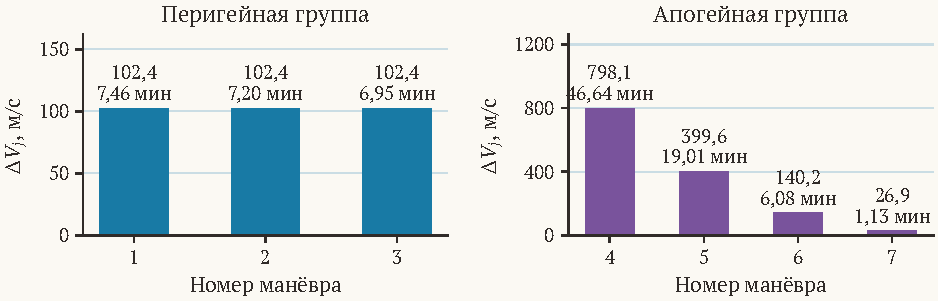
\includegraphics[width=\textwidth,height=40mm,keepaspectratio]{images/kepler-groups-slide.pdf}\par}
\justifying
Равные веса ограничивают наибольший манёвр первой группы.
Убывающая вторая группа оставляет небольшой заключительный манёвр.
\end{frame}

\begin{frame}{Откуда взяты убывающие веса}
\relax
\derivationmathspacing
Исходный требуемый вектор принят за единицу.
После каждого манёвра остаток распределяется между оставшимися манёврами.
\begin{columns}[T,onlytextwidth]
\begin{column}{.50\textwidth}
{\eqcompact\derivationmathspacing
\[
 W_j=\sum_{k=j}^Nw_k,\qquad
 s_j=\frac{w_j}{W_j}\rho_{j-1},\qquad\rho_0=1,
\]
\[
\begin{aligned}
 \rho_j=\bigl[&\rho_{j-1}^2+(1+\eta)^2s_j^2\\
 &-2\rho_{j-1}(1+\eta)s_j\cos\theta\bigr]^{1/2}.
\end{aligned}
\]
}
\justifying
$s_j$ --- плановая величина очередного манёвра,
$\rho_j$ --- требуемый остаток после него;
$\theta,\eta$ --- ошибки направления и величины.
\end{column}
\begin{column}{.47\textwidth}
{\eqcompact\derivationmathspacing
\[
 C(\vect w)=\sum_{j=1}^N(1+\eta)s_j+\rho_N,
\]
\[
 \sum_{j=1}^Nw_j=1,\qquad w_j\geqslant0.
\]
}
При $N=4$, $\theta=3^\circ$, $\eta=0$
минимум $C$ даёт выбранные веса.
\par\smallskip
\justifying
В орбитальном расчёте ошибок исполнения нет;
веса задают демонстрационный профиль групп для пристрелки.
\end{column}
\end{columns}
\end{frame}

\begin{frame}{Размещение манёвров на текущей орбите}
\relax
\derivationmathspacing
\begin{columns}[T,onlytextwidth]
\begin{column}{.49\textwidth}
После предыдущего манёвра:
\[
 P=2\pi\sqrt{\frac{a^3}\mu}.
\]
\begin{enumerate}
\setlength{\itemsep}{5pt}
\item Пассивный прогноз не менее $1{,}5P$;
при переходе ко второй группе --- не менее $2P$.
\item Поиск следующего заданного значения истинной аномалии.
\item Найденное время принимается за $t_c$;
начало $t_b=t_c-\tau/2$.
\end{enumerate}
\end{column}
\begin{column}{.48\textwidth}
{\eqcompact\derivationmathspacing
\[
 \begin{aligned}
 \nu_{c,1}&=0\pmod{2\pi},\\
 \nu_{c,2}&=\pi+\delta\nu\pmod{2\pi}.
 \end{aligned}
\]
\[
 \tau=\frac{m_b c}{F}
 \left(1-e^{-\Delta V/c}\right).
\]
}
\justifying
Сначала $\delta\nu=0$; затем общий сдвиг второй группы
уточняется вместе с величинами и направлениями тяги.
\par\smallskip
Внутри каждой группы используется одно постоянное инерциальное направление.
Времена центров пересчитываются при каждом новом прогнозе.
\end{column}
\end{columns}
\end{frame}

\begin{frame}{Что меняют длительность и $J_2$}
\relax
\derivationmathspacing
Сравнение в общей конечной эпохе $t_f-t_0=10$ суток.
\par\smallskip
{\eqcompact
\centering
\setlength{\tabcolsep}{7pt}
\renewcommand{\arraystretch}{1.12}
% Model comparison; terminal norm is dimensionless.
\begin{tabular}{@{}lrrr@{}}
\toprule
Модель & $\|\mathbf F\|_2$ & $\Delta V_\Sigma$, м/с & $m_f$, кг \\
\midrule
Два импульса & $0$ & 1671{,}943 & 1132{,}973 \\
Протяжённые, центр. поле & $1{,}519\cdot10^{-2}$ & 1671{,}943 & 1132{,}973 \\
Протяжённые, $J_2$ & $2{,}465\cdot10^{-1}$ & 1671{,}943 & 1132{,}973 \\
Уточнённые, $J_2$ & $5{,}927\cdot10^{-11}$ & 1712{,}320 & 1117{,}530 \\
\bottomrule
\end{tabular}
\par
}
\vspace{3.5mm}
\begin{columns}[T,onlytextwidth]
\begin{column}{.48\textwidth}
\textbf{Конечная длительность}
{\eqcompact\derivationmathspacing
\[
 a=\KeplerCentralA\ \text{км},\quad e=\KeplerCentralE,
\]
\[
 i=\KeplerCentralI^\circ.
\]
}
Прежняя $\Delta V_\Sigma$ уже не обеспечивает целевую орбиту.
\end{column}
\begin{column}{.49\textwidth}
\textbf{Дополнительно $J_2$}
{\eqcompact\derivationmathspacing
\[
 \Omega=\KeplerJTwoOmega^\circ,
 \qquad\omega=\KeplerJTwoomega^\circ.
\]
}
\justifying
За время перехода поворачиваются линия узлов и линия апсид.
\end{column}
\end{columns}
\end{frame}

\begin{frame}
\relax
{\centering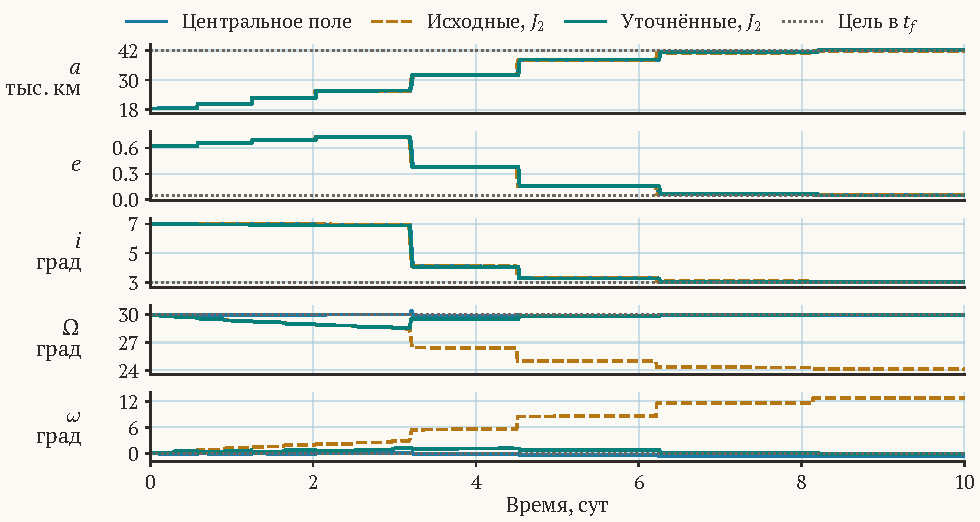
\includegraphics[width=\textwidth,height=80mm,keepaspectratio]{images/kepler-elements-stacked-slide.pdf}\par}
\end{frame}

\begin{frame}{Пристрелка семи протяжённых манёвров}
\relax
\derivationmathspacing
\begin{columns}[T,onlytextwidth]
\begin{column}{.48\textwidth}
\textbf{Семь свободных параметров}
\begin{itemize}
\setlength{\itemsep}{4pt}
\item По три компоненты суммарного приращения скорости каждой группы.
\item Общий сдвиг $\delta\nu$ второй группы.
\end{itemize}
\smallskip
\justifying
Пять условий: поправка наименьшей нормы.
Единицы изменений: $10$ м/с для скорости и $0{,}05$ рад для угла.
\par\smallskip
$\partial\vect F/\partial\vect q$ --- центральными разностями:
по два прогноза на параметр.
\end{column}
\begin{column}{.49\textwidth}
{\centering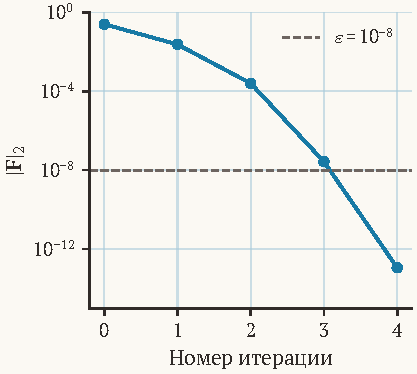
\includegraphics[width=\linewidth,height=44mm,keepaspectratio]{images/kepler-convergence-slide.pdf}\par}
\justifying
Четыре шага; число манёвров и веса сохраняются.
Минимизация расхода топлива здесь не выполняется.
\end{column}
\end{columns}
\end{frame}

\begin{frame}{Найденные величины и направления групп}
\relax
\derivationmathspacing
Характеристические скорости и сдвиг второй группы:
\[
 \Delta V_1=\KeplerTargetGroupOne\ \text{м/с},\qquad
 \Delta V_2=\KeplerTargetGroupTwo\ \text{м/с},\qquad
 \delta\nu=\KeplerSiteShift^\circ.
\]
\begin{columns}[T,onlytextwidth]
\begin{column}{.48\textwidth}
\[
 \vect d_1=\KeplerDirectionOne.
\]
\justifying
Компоненты в опорной ОСК начального перигея двухимпульсного решения.
\end{column}
\begin{column}{.49\textwidth}
\[
 \vect d_2=\KeplerDirectionTwo.
\]
\justifying
Компоненты в опорной ОСК апогея промежуточной орбиты двухимпульсного решения.
\end{column}
\end{columns}
\smallskip
\justifying
Порядок компонент: радиальная, трансверсальная, нормальная.
Опорные базисы фиксируют инерциальные направления;
при интегрировании компоненты пересчитываются в текущую ОСК.
\end{frame}

\begin{frame}{Параметры семи протяжённых манёвров}
\relax
\derivationmathspacing
{\eqcompact
\centering
\setlength{\tabcolsep}{9pt}
\renewcommand{\arraystretch}{1.07}
% Seven final finite-thrust manoeuvres.
\begin{tabular}{@{}rrrrr@{}}
\toprule
№ & $t_{b,j}$, сут & $\tau_j$, мин & $\Delta V_j$, м/с & $m_{e,j}$, кг \\
\midrule
1 & 0{,}574791 & 8{,}1368 & 111{,}950 & 1925{,}325 \\
2 & 1{,}243129 & 7{,}8330 & 111{,}950 & 1853{,}438 \\
3 & 2{,}030448 & 7{,}5406 & 111{,}950 & 1784{,}235 \\
4 & 3{,}186469 & 46{,}5374 & 804{,}959 & 1357{,}140 \\
5 & 4{,}521616 & 18{,}9317 & 403{,}030 & 1183{,}395 \\
6 & 6{,}254308 & 6{,}0494 & 141{,}363 & 1127{,}877 \\
7 & 8{,}200499 & 1{,}1275 & 27{,}116 & 1117{,}530 \\
\bottomrule
\end{tabular}
\par
}
\smallskip
Времена $t_{b,j}$ отсчитываются от $t_0$.
\[
 \Delta V_\Sigma=\KeplerTargetDVTotal\ \text{м/с},\qquad
 \text{увеличение на }\KeplerDVIncrease\ \text{м/с}.
\]
\justifying
Выполнены ограничения: $60\leqslant\tau_j\leqslant3600$ с,
паузы не менее $12$ ч, завершение манёвров до $t_f$.
\end{frame}

\begin{frame}{Траектория перехода}
\relax
{\centering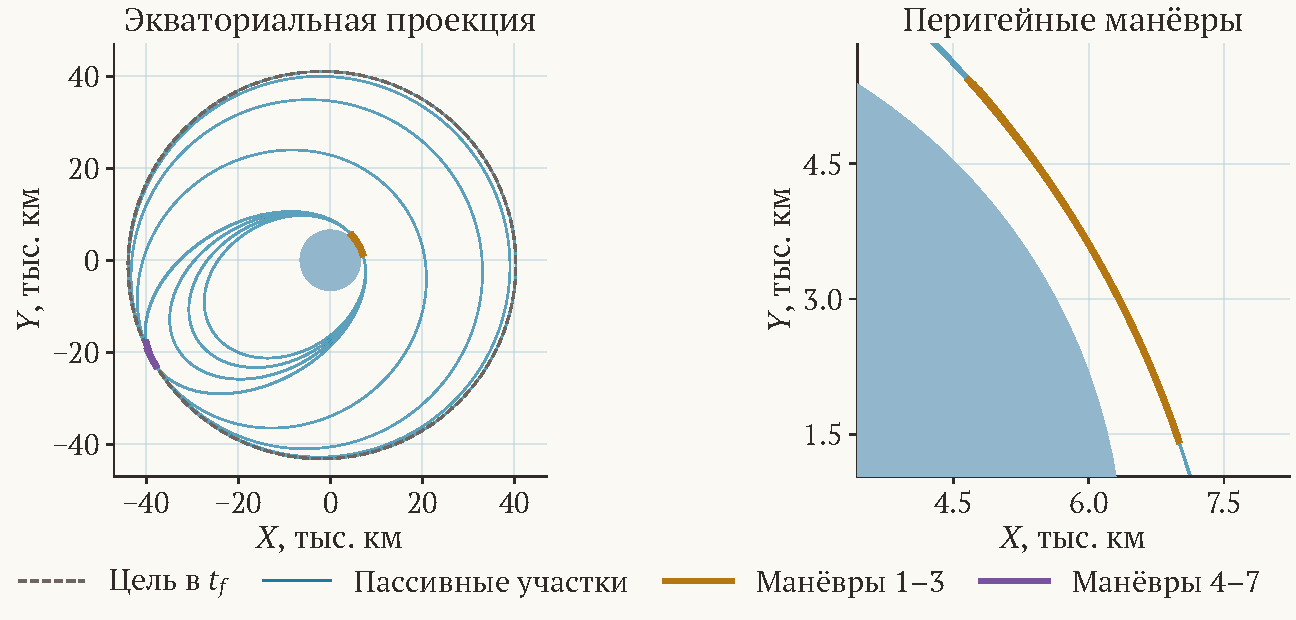
\includegraphics[width=\textwidth,height=62mm,keepaspectratio]{images/kepler-orbit-slide.pdf}\par}
\end{frame}

\begin{frame}{Тяга и масса аппарата}
\relax
\derivationmathspacing
{\centering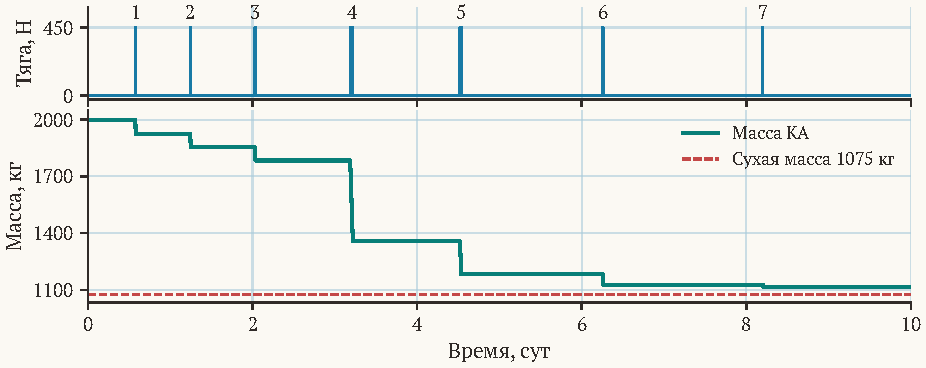
\includegraphics[width=\textwidth,height=44mm,keepaspectratio]{images/kepler-timeline-slide.pdf}\par}
{\eqcompact\derivationmathspacing
\[
 m_f=\KeplerFinalMass\ \text{кг};\qquad
 \text{расход }\KeplerFuel\ \text{кг};\qquad
 \text{запас }\KeplerDryReserve\ \text{кг}.
\]
}
Масса интегрируется во время каждого манёвра;
между манёврами продолжается возмущённое движение.
\end{frame}

\begin{frame}{Полученная орбита и проверка результата}
\relax
\derivationmathspacing
Повторный прогноз с теми же параметрами и более строгими допусками:
\[
 \lVert\vect F\rVert_2=\KeplerNormTight<\varepsilon=10^{-8}.
\]
{\eqcompact
\centering
\setlength{\tabcolsep}{10pt}
\renewcommand{\arraystretch}{1.12}
% Target and attained classical elements; tighter Gauss forecast.
\begin{tabular}{@{}lrr@{}}
\toprule
Элемент & Цель & Повторный прогноз \\
\midrule
$a$, км & 42164{,}000000 & 42164{,}000001 \\
$e$ & 0{,}05000000000 & 0{,}05000000000 \\
$i$, град & 3{,}000000000 & 3{,}000000000 \\
$\Omega$, град & 30{,}000000000 & 29{,}999999999 \\
$\omega$, град & 0{,}000000000 & $-1{,}2896\cdot10^{-9}$ \\
$\nu$, град & Свободна & 111{,}967589 \\
\bottomrule
\end{tabular}
\par
}
\smallskip
\justifying
Пристрелка уточнила величины, направления и положения семи манёвров.
Заданные $a_f,e_f,i_f,\Omega_f,\omega_f$ получены
в общей конечной эпохе; истинная аномалия свободна.
\end{frame}


\begin{frame}{Литература}
\relax
\setbeamertemplate{bibliography item}{\insertbiblabel}
\begin{thebibliography}{9}
\bibitem{diprinzio}
DiPrinzio M. \textit{Methods of Orbital Maneuvering}.
AIAA, 2019. Гл.~11--12: протяжённые манёвры,
структура групп, возмущения и пристрелка.
\bibitem{baranov}
Баранов А.~А. \textit{Маневрирование космических аппаратов
в окрестности круговой орбиты}.
М.: Спутник+, 2016. 511~с.
\end{thebibliography}
\end{frame}
\end{document}
